% !TEX root=dissertationmain.tex
%Chapter
\chapter{Discussion and Results}
\label{discussion}

\paragraph{}In this chapter, the application developed and the thesis as a whole will be reviewed. 
\paragraph{}The aim of this dissertation was to design and develop a proof of concept tool to be utilised by the red teaming individuals such as penetration testers during a security assessment. The application was required to be versatile, portable and reliable allowing it to be used in any size of network topology. From the Application Brief \ref{brief}, the application serves as an additional tool to be used during the initial enumeration stage of a penetration test. It will provide the user with several graphs and statistics on the network which are not provided by currently available commercial tools, such as a visual network overview of machine differences. The application primarily targets are security professionals and network administrators whom want a visual representation of their overall network security due to how well the application scales to network sizes.
\paragraph{}The main findings of this thesis show that red teaming can benefit greatly from machine learning techniques and more research needs to be carried out to move the industry forward towards more accurate, faster and efficient software tools. The results from the proof of concept testing of the application against a network with approximately fifty hosts can be found at Appendix \ref{hacklab} and information on how the test was carried out can be found in section \ref{testing}. The results show that the application was successful in classifying the difference and vulnerability level of the hosts on the network. The following paragraphs will analyse the results in order to show how this conclusion was achieved.
\paragraph{}The application relies on the two scan files used, Nmap and Nessus, for its accuracy as they provide the bases of all the information used for every calculation involved in the software. This means that these two scan files can be used to validate the application results by manually checking each scanner output within their respective applications. \linebreak
\paragraph{}First, the results of the application must be outlined and analysed to then be compared against the files, this is carried out in the following subsection.
\subsection{Test Results Analysis and Validation}
\label{testresults}

\paragraph{}This subsection will summarise the results of the application testing followed by the validation and in depth explanation of those results.

\subsubsection{Analysis of Results}
\label{results_analysis}
\paragraph{}The application detected the five IP addresses in Figure \ref{ips} as the most vulnerable based on their vulnerabilities and properties. This is shown in both the application's GUI output in Figure \ref{results} and its text output in \ref{hacklabtext}: 

\begin{figure}
\label{ips}
\begin{center}
\begin{tabular}{ |c| }
\hline
10.0.0.1\\ \hline
10.0.0.185\\ \hline
10.0.0.3\\ \hline
10.0.0.5\\ \hline
10.0.0.7\\ \hline
\end{tabular}
\end{center}
\caption{The five detected vulnerable IP addresses from the Hacklab Analysis testing section in \ref{testing}}
\end{figure}


\begin{figure}[!h]
\centering
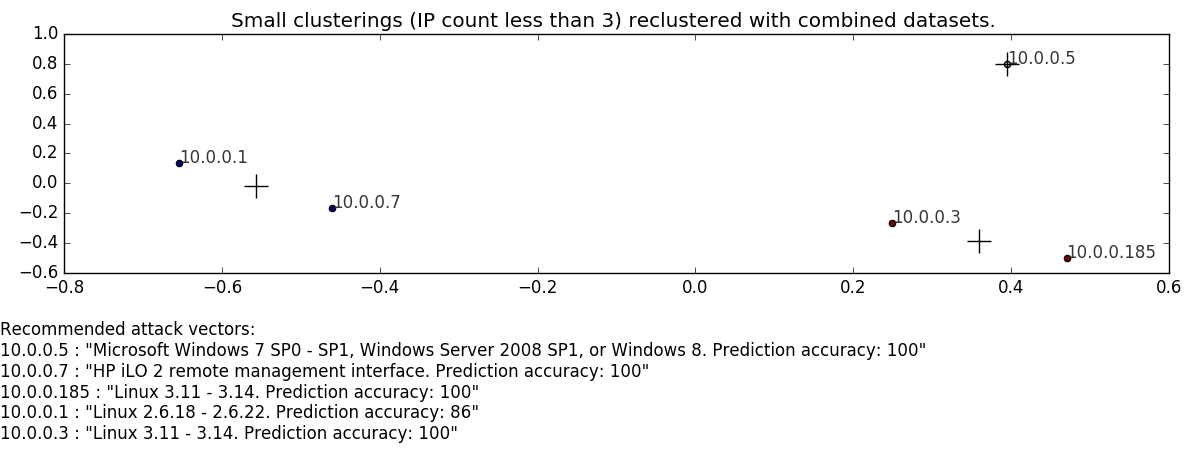
\includegraphics[width=6in]{./Figures/results.png}
\caption{Short excerpt from the application's graphing output in automatic dual mode from Abertay University's Hacklab network analysis \ref{testing}}
\label{results}
\end{figure}

\paragraph{}Figure \ref{results} shows the lower segment of the full results in Figure \ref{dual}, specifically, the vulnerability clustering section of the application explained in \ref{CMFV}. The top graph represents the IP addresses from the small clusters, in this case clusters with less than three IP addresses, clustered via how similar they are to each other and their vulnerability properties, if any were detected by the Nessus scanner. This means that these hosts have the greatest difference from the majority of others in the network and most likely have known vulnerabilities. However, if the majority of hosts on the network have the same vulnerability, then the application will only display the \textit{different} ones, resulting in those hosts not being shown. This scenario is discussed further on in the discussion. 

\paragraph{}From the application's maximum verbosity text output in \ref{hacklabtext}, line 237 shows that the five selected hosts were selected based on 491 different features per host, which was achieved by joining both feature sets together for this part of the application. The features are passed through PCA, similarly to that of the regular clustering section of the application to reduce these 495 features into a two-dimensional dataset. The split for this feature set in this particular test was 288 for Nessus (line 7) and 203 for Nmap (line 11), this relates to a 59\% bias in the clustering towards the Nessus parsed features. Due to Nessus providing all the information about the vulnerabilities and Nmap providing a greater overall amount of system information, the two sets of data work together to give the application a more complete overview of the network. The Nessus bias allows the application to prioritise the vulnerabilities in the clustering algorithm over general system information. However, this ratio is fluid and changes depending on the Nessus configuration used and the networked hosts themselves. This unequal ratio is due to the fact that, while the Nmap scanner returns the same amount of data per machine without variance, the Nessus scanner outputs vary greatly depending on the number and detail of the vulnerabilities detected. This means that a network with a greater number of detailed vulnerabilities on its hosts will provide a much greater clustering bias towards the Nessus data, rather than the Nmap data. This bias only occurs when both data-sets are combined during the final vulnerability detection stage of the application explained in \ref{CMFV} and not during individual tool clustering's. Based off this information, the application recommends these afore mentioned five hosts to be targeted first during a manual security assessment as they will provide the greatest chance of success.

\paragraph{}The text information beneath the graph in Figure \ref{results} shows the operating systems detected for each host in \ref{ips} as well as the probability percentage of this prediction being accurate. The four graphs in figure \ref{results2} represent the other half of the applications output in automatic dual mode. Each graph is titled to show the user what they each represent. As mentioned previously these clustering's use their respectable tool files and thus, do not contain the bias that Figure \ref{results} has. Two of these four graphs are the exact same as those found if the application were to execute using the single dataset mode for each tool as such demonstrated in Figures \ref{split_nessus} and \ref{split_nmap}. This section of the output can be found explained in section \ref{display}. The IP addresses of hosts in Figure \ref{ips} can be seen within the two clustering's, showing how those hosts relate to the other hosts of larger clusters, in the same terms as Figure \ref{results} but keeping the tool output features to their individual graphs.

\begin{figure}[!h]
\centering
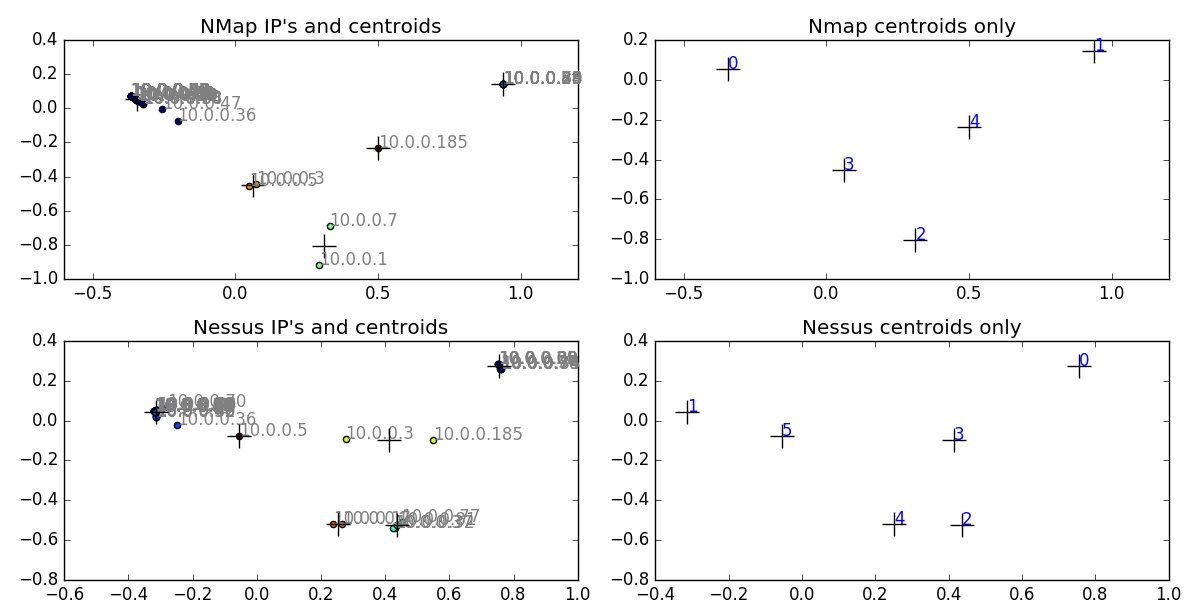
\includegraphics[width=6in]{./Figures/results2.png}
\caption{standard tool output graphs from application's graphing output in automatic dual mode from Abertay University's Hacklab network analysis \ref{testing}}
\label{results2}
\end{figure}

\subsubsection{Validation}

\paragraph{}In order to determine whether the detected IP addresses in Figure \ref{ips} are that of the most differential hosts, each tool output must be investigated individually. By uploading the Nessus file onto a Nessus web interface of version 6 or above, it is possible to see an overview of the file with colour coded bars for each host. This is represented in Appendix Figures \ref{hacklab_nessus1} and \ref{hacklab_nessus2}. The original image was split into two Figures simply due to the size being too large for this paper. The key for the colour coded bars in the Nessus overview is as follows:
\begin{center}
\begin{tabular}{ |c|c| }
\hline
Red & Critical rank vulnerability\\ \hline
Yellow & Medium rank vulnerability\\ \hline
Green & Low rank vulnerability\\ \hline
Blue & Host information\\ \hline
\end{tabular}
\end{center}

\paragraph{}Through analysis of the Nessus overview using the key above, the differences in vulnerabilities per host are made apparent as visually intended by the developer, Tenable\textsuperscript{TM}. By specifically viewing the selected hosts in this overview, it can be observed that \textbf{they are indeed, the most unique compared to the other hosts} in terms of Critical, Medium and Low ranked vulnerabilities. When using this method to compare hosts, it is important to not provide as much weight to the key colour blue representing the host information as to the vulnerability codes. This is because the blue host information is given much lower importance than the vulnerabilities in the Nessus parser class. If the keys shown above were weighted equally, the clustering would not have the bias towards the vulnerabilities and result in a less accurate prediction by the algorithm. Unfortunately, there is no similar visualisation method to validate the Nmap graph and requires manually reading the output XML file and comparing It to the application graphs.

\paragraph{}Another method to validate the network is a manual approach, which requires in-depth prior knowledge of the network used. This approach is possible for individuals such as network administrators who might use this tool for the purpose of confirming the results of a security assessment, and not to discover new information. This approach is not possible for scenarios such as capture the flag events where there is no prior knowledge of the network and its hosts. The manual approach involves comparing the application's verbose text output, such as each cluster's shared features, to the individual's prior knowledge of the network. The following section will give a critical evaluation of the application.

\subsection{Critical Evaluation}
\label{criteval}
\paragraph{}This section will provide a short critical evaluation of the application and its performance in its intended role.

\paragraph{}As previously mentioned in this discussion, if the used network contains a large number of hosts with the same vulnerability, then those hosts become the majority and since the application, in its essence, finds the differences in hosts, the clustering might not reflect the hosts with that vulnerability accurately. This problem is difficult to solve completely as it would involve changing the application's core design architecture. A possible untested solution however, is as follows. By adding a new layer on top of the parser classes to make it aware of common vulnerabilities in the dataset, then displaying them to the user directly would mitigate this problem. Another possible workaround is simply for the user to manually check for any common, major vulnerabilities within the Nessus overview as mentioned in the previous section and take them into account when considering the application's results.

\paragraph{}Unfortunately, due to the nature of the datasets used including sensitive information, there are no online datasets that the application could use. This makes the creation of a proper testing procedure difficult as all data used for this application within this project was created specifically for this project. This means that the application is to be taken simply as a proof of concept and not a finalised design.

\paragraph{}Due to project time constraints, the primary automatic dual mode of the application was only able to be implemented with the K-means algorithm however, both DBscan and agglomerative implementations are already fully programmed and integrated into the model. The only issue stopping these algorithms to be integrated into this mode is the fact the sklearn python library (used to calculate several of the clustering functions) does not include centroid support for them and one would have to be manually programmed, which would take more time than was available for the project. Once that feature has been implemented, the two algorithms can be re-enabled with minimal difficulty.

\paragraph{}The application has been optimised for model prediction accuracy over performance times, however, each class module within the application has been programmed modularly allowing for the easy modification by others without prior knowledge of how it was created. Variables may be changed easily, such as the IP cut off limit for the vulnerability detection stage explained in \ref{CMFV} without fear of it causing problems elsewhere in the application. Another such example of modularity is allowing the option of modifying the parsing classes to change what it taken as features and labels from each tool output. When using a network with less than a hundred hosts such as that of in the testing chapter, the application will take between one and three minutes to complete on the dual automatic mode. Other modes such as manual and assisted can be completed in less than thirty seconds. This performance could be improved by converting parts of the application models to a language such as C++ although this would greatly reduce the customization level of the application, which is one of the primary design features. Upon successful completion of the clusterer, the application will write to two files. One of which is a dot file including the primary clustering and the other is a target file including the selected hosts from the results. The latter file can be imported into many tools such as Metasploit and Armitage to manually assess those hosts. The former can be imported into graphing tools such as Gephi to interface with them in a different manner than the integrated interface. Both these output files can be easily disabled they are not needed by modifying one line at the end of the initialization class.

\subsection{Discussion Summary}
\paragraph{}The findings in this thesis contribute towards developing a machine learning arsenal of tools that can be used by security professionals, as well as help balance the research in the security industry by providing a unique red teaming proof of concept tool. The results of the testing are of direct practical relevance to the red team, and such align with the design goals highlighted in \ref{brief}. Only a couple of other studies, to our knowledge, have examined the use of machine learning in red teaming. It is clear that further research in this area is necessary before machine learning can become common place in this industry sector, however, this paper has helped cleared ground for this research to take place in. This paragraph marks the end of the discussion and the following section will provide conclusions to the paper.
